\documentclass[11pt]{article}

\usepackage{tocloft}
\usepackage[margin=1in]{geometry} %used for margins
\usepackage{graphics}
\usepackage{graphicx}
\usepackage{gensymb} %for symbols such as the degree sign
\usepackage{titlesec}
\graphicspath{
{figures/}
{../figures/}
{../../figures/}
{../../figures/screenshots/}
{../../figures/plots/}
}
\usepackage[natbibapa]{apacite}
% \usepackage[]{natbib}
\usepackage{xcolor}
\usepackage{array}% http://ctan.org/pkg/array
\usepackage{tikz} %used for drawing colored boxes 
\usepackage{bibentry} %for full citations
% \nobibliography* 
\usepackage{subfig} %for creating panels
\usepackage{todonotes}  
\usepackage{longtable}  
\usepackage{booktabs}% http://ctan.org/pkg/booktabs
\usepackage[countmax]{subfloat} %for creating panels
\usepackage{enumitem} %better environment for lists 
\usepackage{multirow} %to have multiple row entries in tables 
\usepackage{breakurl} %to break urls
\usepackage{wrapfig} %to wrap figures
\usepackage{float}  %for floating figures
\usepackage{amsmath}
\usepackage{hyperref} %to h ave links within the document 
\hypersetup{
    colorlinks,%
    citecolor=black,%
    filecolor=black,%
    linkcolor=black,%
    urlcolor=black
}

%to allow for more figures per page 
\renewcommand\floatpagefraction{.95}
\renewcommand\topfraction{.95}
\renewcommand\bottomfraction{.95}
\renewcommand\textfraction{.05}   
\setcounter{totalnumber}{50}
\setcounter{topnumber}{50}
\setcounter{bottomnumber}{50}

%some settings to make lists look nicer 
\setlist{leftmargin=*} 
\setlist[1]{labelindent=\parindent} % Only the level 1
\setlist{topsep = 0cm,partopsep = 1pt, parsep = 1pt} %changes the separation of lists 

%some stuff to decrease the space around section headings, etc. 
\titleformat{\section}
  {\bfseries \Large}{\thesection}{0.5em}{}

\titleformat{\subsection}
  {\bfseries \large}{\thesubsection}{0.5em}{}

\titleformat{\subsubsection}
{\bfseries}{\thesubsubsection}{0.5em}{}

\titlespacing{\section}{0cm}{0.3cm}{0.1cm}
\titlespacing{\subsection}{0cm}{0.3cm}{0.1cm}
\titlespacing{\subsubsection}{0cm}{0.3cm}{0.1cm}

%special trick for having vertically aligned table entries (just use M instead of the normal ways of defining table columns)
\newcolumntype{M}{>{\centering\arraybackslash}m{\dimexpr.2\linewidth-2\tabcolsep}}

%command to create boxes 
\newcommand{\mycbox}[2]{\tikz{\path[draw=#1,fill=#2] (0,0) rectangle (1cm,1cm);}}

%nice to do notes
\newcommand{\sttodo}[2][]
{\todo[caption={\textbf{TG}}, size=\small, color = orange, #1]{#2}~}
\newcommand{\ttodo}[2][]
{\vspace{0.1cm}\hfil \todo[caption={\textbf{TG}}, size=\small, color = orange, inline, #1]{#2}}

%for tick marks
\usepackage{pifont}% http://ctan.org/pkg/pifont
\newcommand{\cmark}{\ding{51}}%
\newcommand{\xmark}{\ding{55}}%

%for possessive citing
\def\citepos#1{\citeauthor{#1}'s (\citeyear{#1})}

\begin{document}

\begin{center} 
{\LARGE \textbf{Tug of war}}
\linebreak
% \linebreak
% {\large Tobias Gerstenberg (\href{mailto:tger@mit.edu}{tger@mit.edu})}
\linebreak
\today
\end{center} 

\tableofcontents 

\clearpage 

\section{Research question}
\label{sec:research_question}

\begin{itemize}
	\item exploring the probabilistic language of thought hypothesis as a model for human inference in tug of war world
	\item demonstrate compositionality and productivity of thought 
\end{itemize}

\section{Experiment 1: How strong?}
\label{sec:experiment_1_how_strong}

{\setlength{\tabcolsep}{2pt} 
% \begin{longtable}{@{\extracolsep{\fill} } cccc}
\begin{longtable}{cccc}

\caption{Games used in Experiment~1. Participants were always asked about the strength of player 1. \emph{Note}: $>$ indicates that team1 won against team2; $<$ indicates that team1 lost against team2.}\\

  \toprule
 id & team1 & winner & team2 \\
  \midrule
  \endfirsthead

  \toprule
 id & team1 & winner & team2 \\
  \midrule
  \endhead
1 & 1 & $>$ & 2 \\ 
  1 & 1 & $>$ & 2 \\ 
  1 & 1 & $>$ & 2 \\ 
\midrule
  2 & 1 & $>$ & 2 \\ 
  2 & 2 & $>$ & 3 \\ 
  2 & 2 & $>$ & 4 \\ 
  \midrule
  3 & 1 & $>$ & 2 \\ 
  3 & 2 & $<$ & 3 \\ 
  3 & 2 & $<$ & 4 \\ 
  \midrule
  4 & 1 & $>$ & 2 \\ 
  4 & 1 & $>$ & 3 \\ 
  4 & 1 & $>$ & 4 \\ 
  \midrule
  5 & 1,2 & $>$ & 3,4 \\ 
  5 & 1,2 & $>$ & 5,6 \\ 
  5 & 1,2 & $>$ & 7,8 \\ 
  \midrule
  6 & 1,2 & $>$ & 5,6 \\ 
  6 & 1,3 & $>$ & 5,7 \\ 
  6 & 1,4 & $>$ & 5,8 \\ 
  \midrule
  7 & 1,2 & $>$ & 5,6 \\ 
  7 & 2,3 & $<$ & 5,6 \\ 
  7 & 2,4 & $<$ & 5,6 \\ 
  \midrule
  8 & 1,2 & $>$ & 5,6 \\ 
  8 & 2,3 & $>$ & 5,6 \\ 
  8 & 2,4 & $>$ & 5,6 \\ 
  \midrule
  9 & 1,2 & $>$ & 5,6 \\ 
  9 & 1,3 & $>$ & 7,8 \\ 
  9 & 1,4 & $>$ & 9,10 \\ 
  \midrule
  10 & 1,2 & $>$ & 3,4 \\ 
  10 & 1,3 & $>$ & 2,4 \\ 
  10 & 1,4 & $>$ & 2,3 \\ 
  \midrule
  11 & 1 & $<$ & 2 \\ 
  11 & 1 & $<$ & 2 \\ 
  11 & 1 & $<$ & 2 \\ 
  \midrule
  12 & 1 & $<$ & 2 \\ 
  12 & 2 & $<$ & 3 \\ 
  12 & 2 & $<$ & 4 \\ 
  \midrule
  13 & 1 & $<$ & 2 \\ 
  13 & 2 & $>$ & 3 \\ 
  13 & 2 & $>$ & 4 \\ 
  \midrule
  14 & 1 & $<$ & 2 \\ 
  14 & 1 & $<$ & 3 \\ 
  14 & 1 & $<$ & 4 \\ 
  \midrule
  15 & 1,2 & $<$ & 3,4 \\ 
  15 & 1,2 & $<$ & 5,6 \\ 
  15 & 1,2 & $<$ & 7,8 \\ 
  \midrule
  16 & 1,2 & $<$ & 5,6 \\ 
  16 & 1,3 & $<$ & 5,7 \\ 
  16 & 1,4 & $<$ & 5,8 \\ 
  \midrule
  17 & 1,2 & $<$ & 5,6 \\ 
  17 & 2,3 & $>$ & 5,6 \\ 
  17 & 2,4 & $>$ & 5,6 \\ 
  \midrule
  18 & 1,2 & $<$ & 5,6 \\ 
  18 & 2,3 & $<$ & 5,6 \\ 
  18 & 2,4 & $<$ & 5,6 \\ 
  \midrule
  19 & 1,2 & $<$ & 5,6 \\ 
  19 & 1,3 & $<$ & 7,8 \\ 
  19 & 1,4 & $<$ & 9,10 \\ 
  \midrule
  20 & 1,2 & $<$ & 3,4 \\ 
  20 & 1,3 & $<$ & 2,4 \\ 
  20 & 1,4 & $<$ & 2,3 \\ 
  \midrule
  21 & 1,2 & $>$ & 3 \\ 
  \midrule
  22 & 1 & $<$ & 2,3 \\ 
  \midrule
  23 & 1,2 & $>$ & 4,5,6 \\ 
  23 & 2 & $>$ & 4,5 \\ 
  \midrule
  24 & 1,4 & $>$ & 5,2,3 \\ 
  24 & 1,5 & $>$ & 2,3,4 \\ 
  \midrule
  25 & 1,2,3 & $>$ & 4,5,6 \\ 
  25 & 2,3 & $>$ & 4,5,6 \\ 
  \midrule
  26 & 1,2 & $<$ & 3 \\ 
  \midrule
  27 & 1 & $>$ & 2,3 \\ 
  \midrule
  28 & 1,2 & $<$ & 4,5,6 \\ 
  28 & 2 & $<$ & 4,5 \\ 
  \midrule
  29 & 1,4 & $<$ & 5,2,3 \\ 
  29 & 1,5 & $<$ & 2,3,4 \\ 
  \midrule
  30 & 1,2,3 & $<$ & 4,5,6 \\ 
  30 & 2,3 & $<$ & 4,5,6 \\ 
 \bottomrule
\end{longtable}
}

\subsection{Methods}
\label{sub:methods}

\subsubsection{Design}
\label{ssub:design}

\subsubsection{Procedure}
\label{ssub:procedure}

\begin{figure}[H]
	\centering
	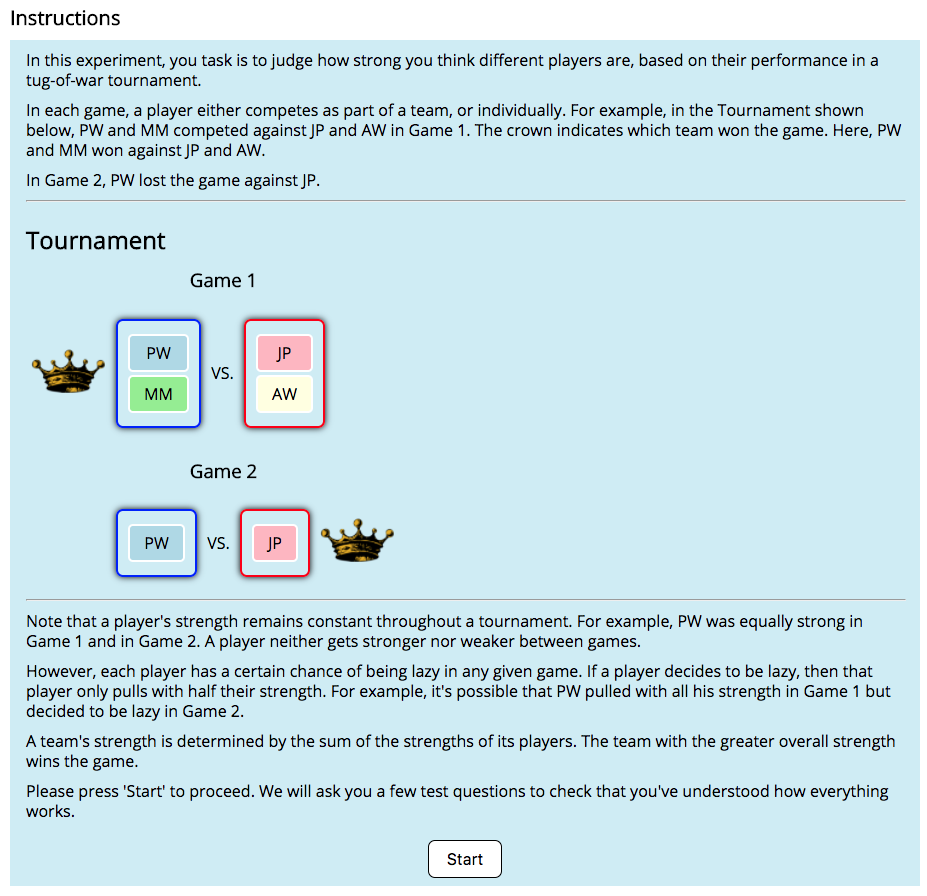
\includegraphics[width=0.5\textwidth]{exp1_screenshot1}
	\caption{Instructions.}
	\label{fig:exp1_screenshot1}
\end{figure}

\begin{figure}[H]
	\centering
	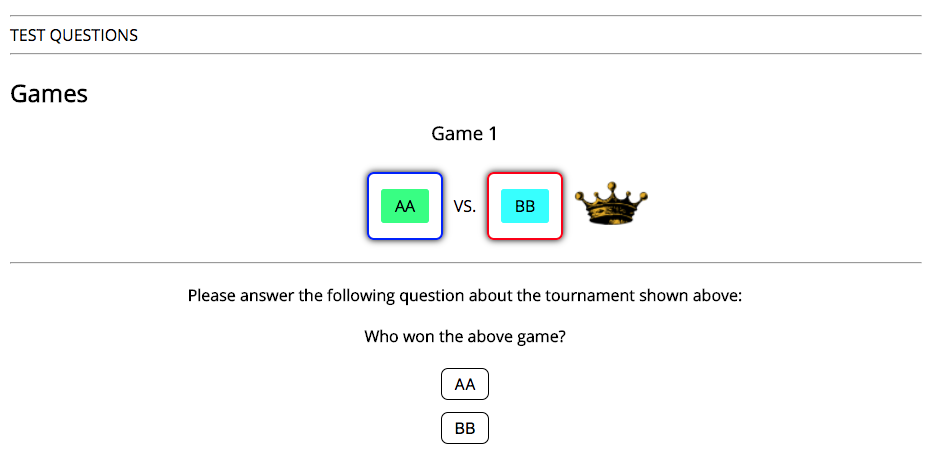
\includegraphics[width=0.5\textwidth]{exp1_screenshot2}
	\caption{Test question.}
	\label{fig:exp1_screenshot2}
\end{figure}

\begin{figure}[H]
	\centering
	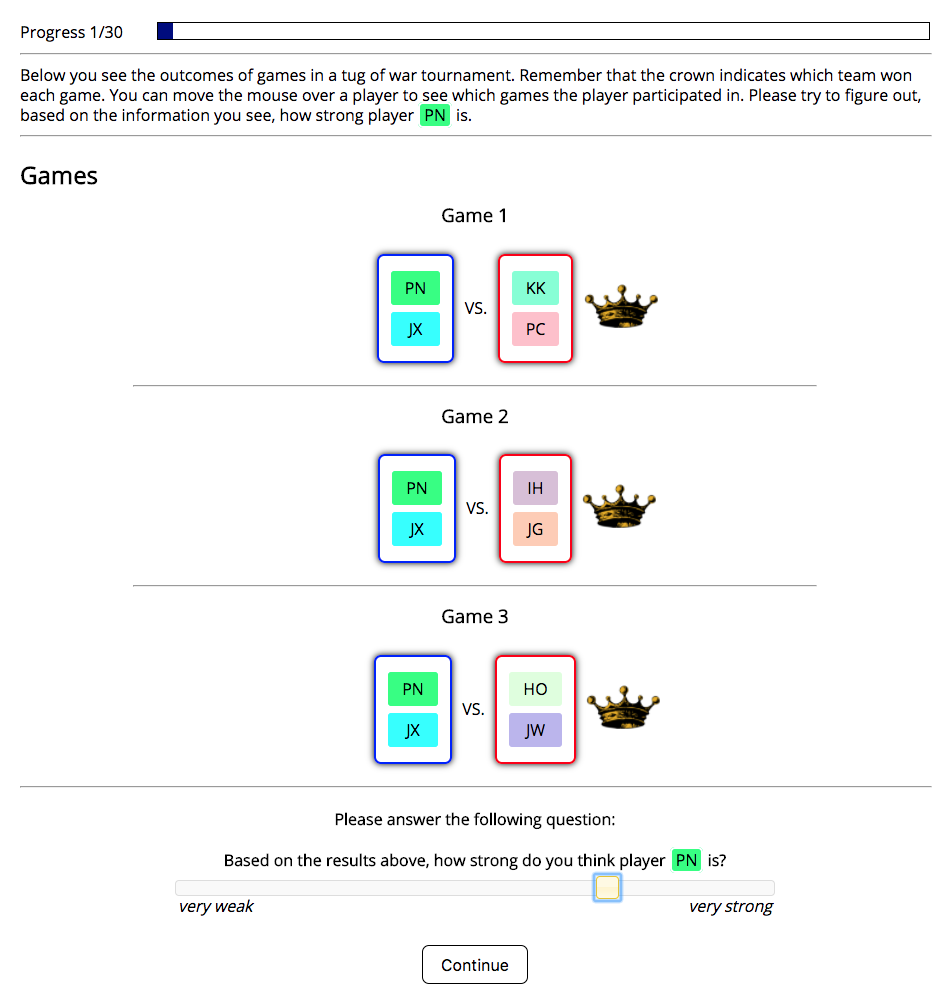
\includegraphics[width=0.5\textwidth]{exp1_screenshot3}
	\caption{Trial.}
	\label{fig:exp1_screenshot3}
\end{figure}

\subsection{Results (N = 39)}
\label{sub:results}

% \begin{figure}[H]
%   \centering
%   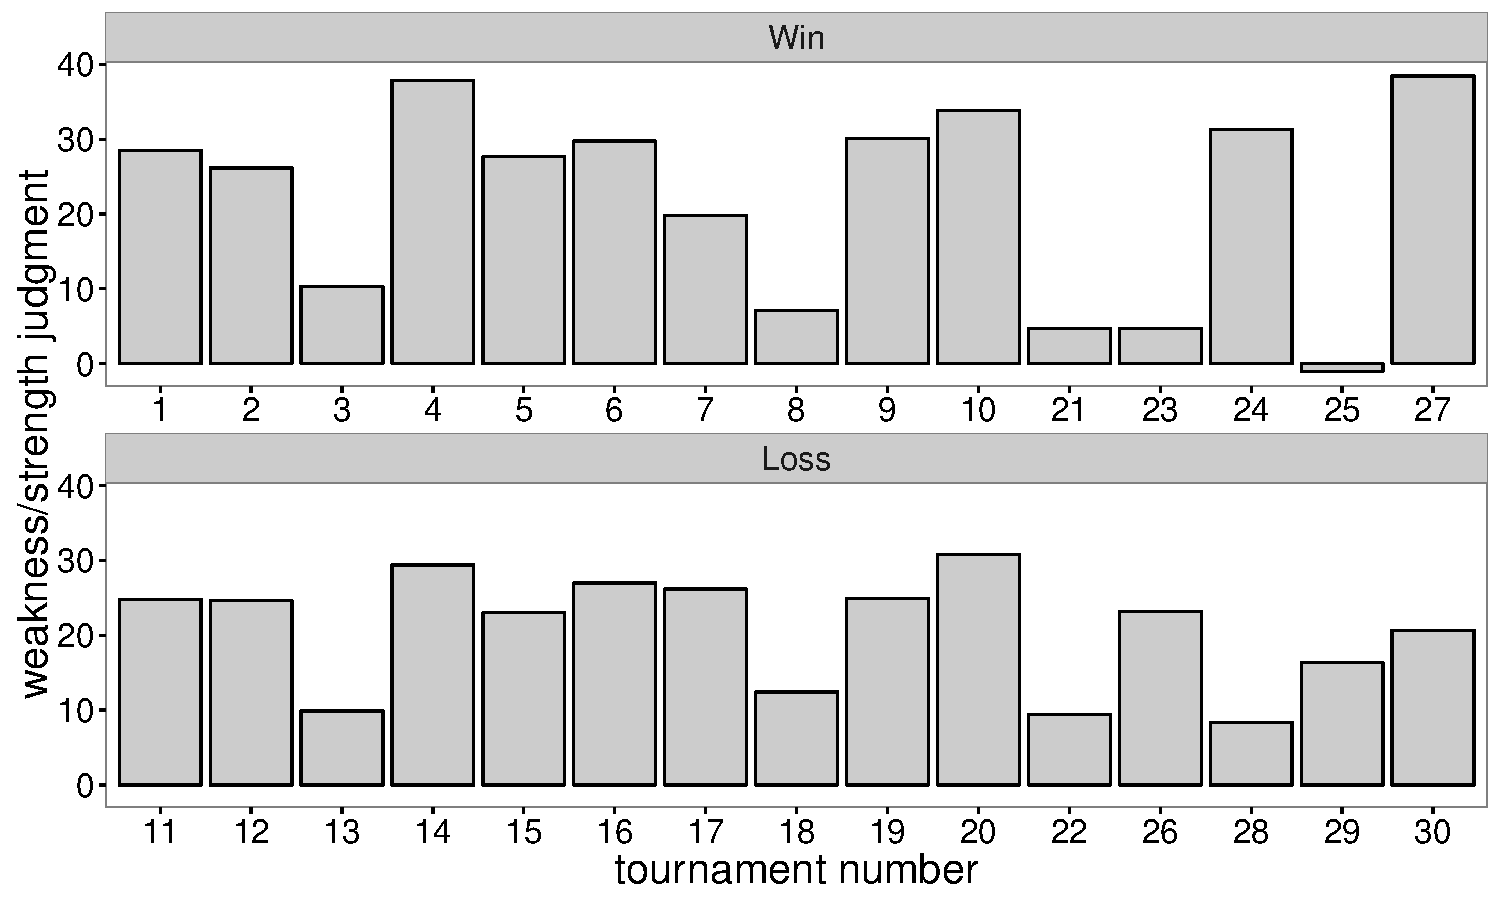
\includegraphics[width=0.95\textwidth]{exp1_bars}
%   \caption{Mean weakness/strength judgments across the 30 tournaments. \emph{Note}: Error bars indicate 95\% confidence intervals.}
%   \label{fig:exp1_bars}
% \end{figure}

\begin{figure}[H]
  \centering
  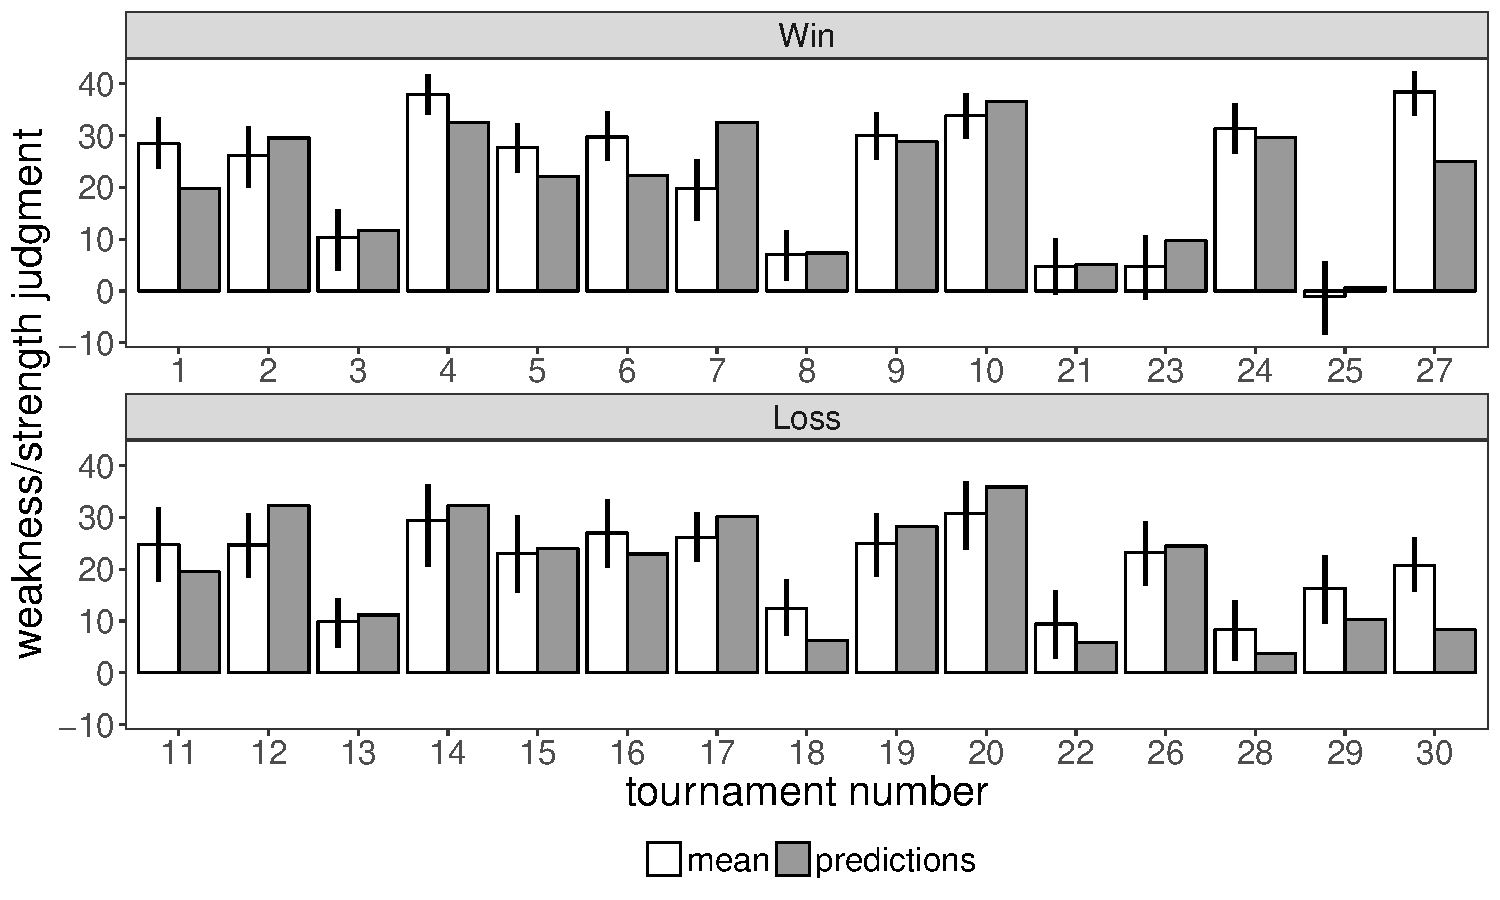
\includegraphics[width=0.95\textwidth]{exp1_data_model_bars}
  \caption{Mean weakness/strength judgments across the 30 tournaments with model predictions. \emph{Note}: Error bars indicate 95\% confidence intervals.}
  \label{fig:exp1_data_model_bars}
\end{figure}

\section{Experiment 2: Asking many questions}
\label{sec:experiment_2_asking_many_questions}

\section{Experiment 3: The omniscient commentator}
\label{sec:experiment_3_the_omniscient_commentator}

\section{Experiment 4: How much effort?}
\label{sec:experiment_4_how_much_effort}

\clearpage
\bibliographystyle{apacite}
\bibliography{references}
\end{document}